% !TeX root = ../../../金融经济学_王江_讲义及习题.tex
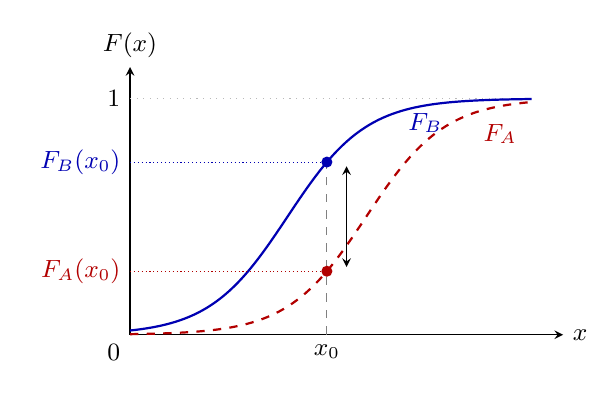
\begin{tikzpicture}[x=1cm,y=1cm,>=stealth,font=\small]
 \path[use as bounding box] (-1.3,-0.65) rectangle (5.8,3.9);
 \draw[->] (0,0)--(5.5,0) node[right] {$x$};
 \draw[->] (0,0)--(0,3.4) node[above] {$F(x)$};
 \node[below left] at (0,0) {$0$};
 \draw[gray!55,dotted] (0,3)--(5.1,3);
 \node[left] at (0,3) {$1$};
 \draw[blue!70!black,thick,domain=0:5.1,samples=90]
   plot (\x,{3/(1+exp(-2*(\x-2)))});
 \draw[red!70!black,thick,dashed,domain=0:5.1,samples=90]
   plot (\x,{3/(1+exp(-2*(\x-3)))});
 \node[blue!70!black,below] at (3.75,2.94) {$F_B$};
 \node[red!70!black,below] at (4.7,2.8) {$F_A$};
 \draw[gray,dashed] (2.5,0)--(2.5,2.1932);
 \draw[blue!70!black,densely dotted] (0,2.1932)--(2.5,2.1932);
 \draw[red!70!black,densely dotted] (0,0.8068)--(2.5,0.8068);
 \fill[blue!70!black] (2.5,2.1932) circle (2pt);
 \fill[red!70!black] (2.5,0.8068) circle (2pt);
 \node[left,blue!70!black] at (0,2.1932) {$F_B(x_0)$};
 \node[left,red!70!black] at (0,0.8068) {$F_A(x_0)$};
 \node[below] at (2.5,0) {$x_0$};
 \draw[<->] (2.75,0.86)--(2.75,2.14);
\end{tikzpicture}%
